%!TEX root = ../dokumentation.tex

\chapter{Architektur}
In den folgenden Kapiteln wird der architekturische Aufbau anhand des in Abbildung \ref{fig:architektur} dargestellten Architekturübersichtsdiagramm 
erläutert. Hierbei wird auf die jeweiligen Architektur-Layer eingegangen und erklärt, welche Eigenschaften die abgebildeten Geräte und Protokolle im Rahmen 
der \ac{IoT}-Lösung mit sich bringen.
\\

\begin{figure}[!htbp]
    \centering
    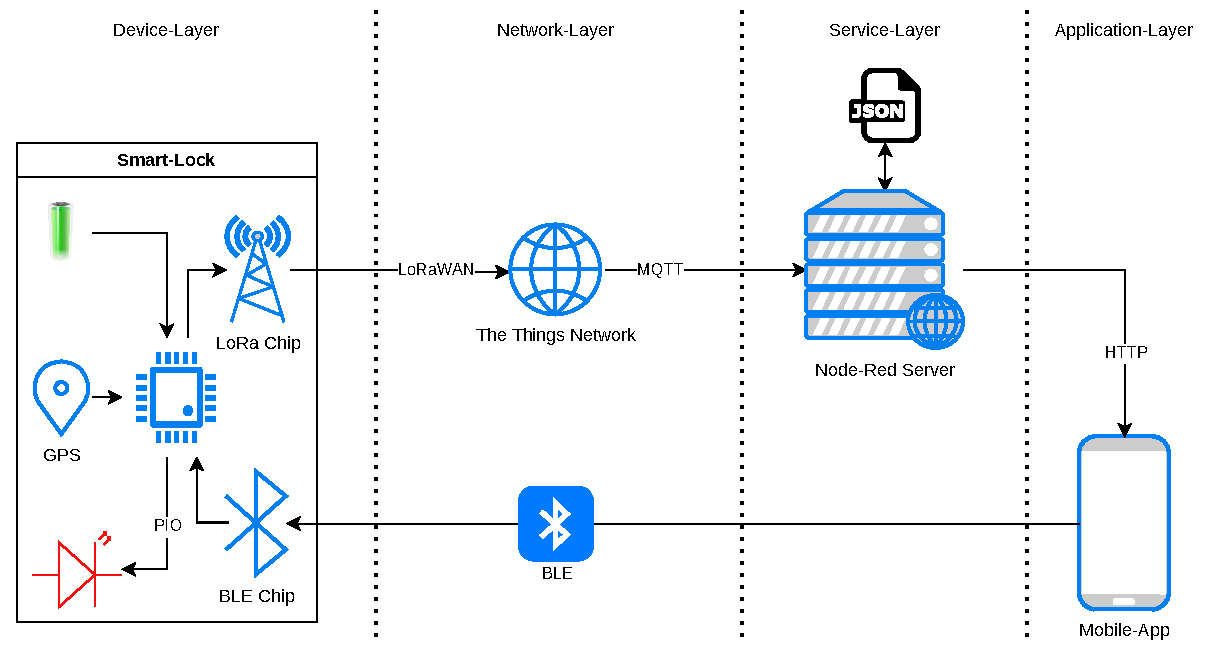
\includegraphics[width=1\linewidth]{images/architecture_smart_lock.pdf}
    \caption[Architektur-Diagram des Smart-Locks]{Architektur-Diagram des Smart-Locks}
    \label{fig:architektur}
\end{figure}

%!TEX root = ../../dokumentation.tex

\section{Device-Layer}
\todo{Hier anfangen zu schreibefn}
%!TEX root = ../../dokumentation.tex

\section{Network-Layer} \label{network}
Das Network-Layer beschreibt die Protokolle und Netzwerk-Server, die die \ac{IoT}-Lösung zum Austausch der Daten verwendetet. Dabei wird in der vorgestellten Lösung auf vier verschiedene übertragungstechnologien gesetzt.

Für die Übertragung der \ac{GPS}-Daten wird \textbf{\ac{LoRaWAN}} verwendet und sendet die Daten an ein Gateway. Das Gateway ist Teil des \ac{TTN}s, ein zusammenschluss aus vielen öffentlichen \ac{LoRaWAN}-Gateways. Im \ac{TTN} werden die Daten über einen Parser in ein \ac{JSON}-Format gebracht und können über herkömmliche Netzwerkprotokolle, wie \ac{HTTP}-WebSockets oder \ac{MQTT} an einen Server übertragen werden.

Die vorgestellte Smart Lock Lösung verwendet für die weitere Übertragung an das Service-Layer \textbf{\ac{MQTT}}. Das hat den Vorteil, dass sich Nachrichten sobald sie Empfangen werden, an den Server übertragen lassen und nicht über ein Request-Response verfahren abgefragt werden müssen. 

Zusätzlich zu \ac{LoRaWAN} und \ac{MQTT} wird in der Lösung \textbf{\ac{HTTP}} für die Kommunikation von App und Server verwendet. Hierfür sendet die Benutzer-App eine \ac{HTTP}-Request an den Node-Red Server, der die Anfrage verarbeitet und die Device-Daten an die App zurücksendet. 

Zuletzt wird \textbf{\ac{BLE}} für das Öffnen und Schließen des Schlosses und somit für die direkte Kommunikation von App zu Device verwendet. \ac{BLE} hat zwei entscheidende Vorteile: geringer Energieverbrauch und geringe Reichweite. Ersteres ist notwendig, damit das Schloss möglichst lange Akkulaufzeiten hat und zweiteres damit das Schloss nur aus unmittelbarer Nähe geöffnet oder geschlossen werden kann.

Zusammengefasst, deckt das Network-Layer die Kommunikation von allen verwendeten Hardware- und Software-Modulen ab und verwendet hierfür \ac{LoRaWAN} über das \ac{TTN} als Gateway zu \ac{MQTT}, sowie \ac{HTTP} und \ac{BLE} für die Kommunikation zur Benutzer-App.
%!TEX root = ../../dokumentation.tex

\section{Service-Layer}
Der Service-Layer besteht aus einem Node-Red Server, der in einem Docker-Container läuft. Das hat den Vorteil, dass die Anwendung beliebig umgezogen oder skaliert werden kann. Zusätzlich empfängt der Server die Daten aus dem \ac{TTN} über \ac{MQTT} und speichert sie lokal in der \emph{Kontext}-Variablen und persistent als \ac{JSON}-Dokument ab. Dadurch können die Daten auch nach einem Neustart der Anwendung weiter verwendet werden. Abbildung \ref{fig:node-red} zeigt die folgenden drei Prozesse in Node-Red:

\begin{itemize}
    \item \textbf{Initialisierung}: Der erste \emph{Flow}, der beim Serverstart einmalig ausgeführt wird. Er lädt das gespeicherte \ac{JSON}-Dokument und setzt die \emph{Kontext}-Variablen auf die gespeicherten Werte.
    \item \textbf{Verbindung zum \ac{TTN}-Server}: Dieser Prozess wird für jede im \ac{TTN} empfangene und weitergeleitete Nachricht ausgeführt und speichert die empfangenen \ac{GPS}- und Sensor-Informationen im \ac{JSON}-Dokument bzw. Kontext des Servers.
    \item \textbf{App Anfrage}: Für jede empfangene \ac{HTTP}-Anfrage an die Route \emph{server-adresse:1880/device-id} wird der \emph{Flow} ausgeführt. Er lädt die Daten für die mitgelieferte \emph{device-id} und schickt sie als Antwort zurück an die App.
\end{itemize}

\begin{figure}[!htbp]
    \centering
    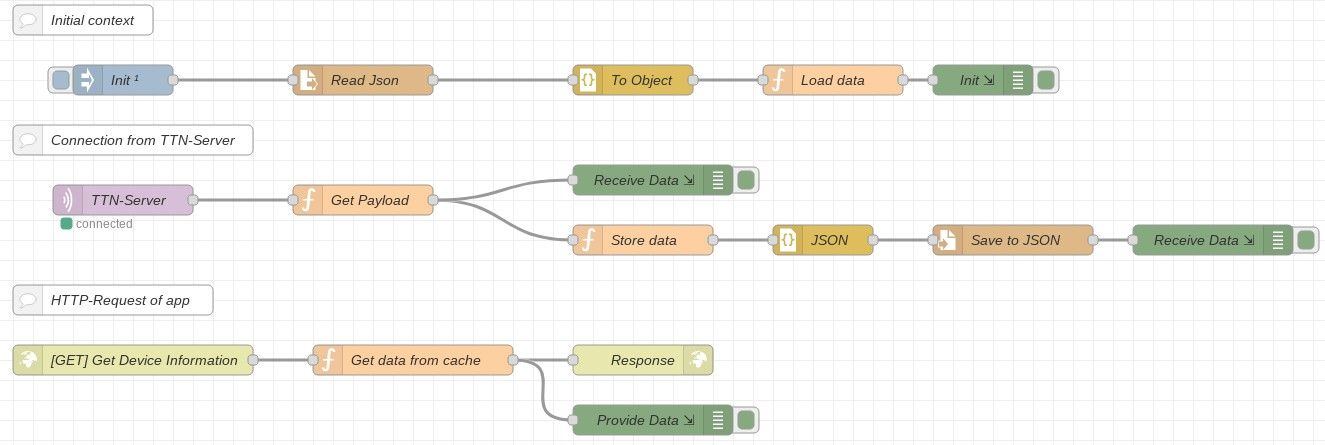
\includegraphics[width=1\linewidth]{images/node-red.jpg}
    \caption[Node-Red Serverarchitektur für das Smart-Lock]{Node-Red Serverarchitektur für das Smart-Lock}
    \label{fig:node-red}
\end{figure}

Außerdem wird der Server in der Azure-Cloud auf einem Ubuntu-Server gehostet. Dadurch ist der Server aus dem Internet zugänglich und die Daten können jederzeit vom Benutzer abgerufen werden.

Zusammengefasst deckt der Server den Service-Layer mit persistenter Speicherung ab, indem er Nachrichten aus dem Network-Layer empfängt und an das Application-Layer weiterleitet. Zusätzlich werden die Daten im Server gespeichert, um sie jederzeit abfragen zu können, auch wenn der Server neu gestartet wurde. In Zukunft lässt sich das System weiter skalieren oder auf einem eigenen Server hosten, da es in einem Docker-Container läuft.
%!TEX root = ../../dokumentation.tex

\section{Application-Layer}
Die vierte Schicht des \ac{IoT}-Application Stack ist der Application Layer. Im Application Layer geht es darum, die vernetzten Geräte für den Nutzer verwendbar zu machen. Hierfür werden Applikationen entwickelt. Im Falle des \ac{IoT} Smart-Lock sollte dies eine Handy-Applikation sein, welche die Kommunikation des Nutzers mit dem Schloss ermöglicht.

Die Anforderungen an die App sind recht simpel: Der Nutzer soll die Schlösser in der App angezeigt bekommen und nahegelegene Schlösser entsperren können. Die Anzeige soll zweigleisig ermöglicht werden. Einerseits soll eine simple Liste die Schlösser aufführen. Zusätzlich soll auch eine Karte die Geo-Positionen der Schlösser mit hoher Genauigkeit anzeigen, um speziell dem Verlustpotential entgegenzuwirken. Der Nutzer soll nahegelegene Schlösser entsperren können. Der Zusatz nahegelegen ist hierbei wichtig, da die Ver- bzw. Entriegelung des Schlosses aus großer Distanz nicht möglich sein soll.

Die App setzt genau obige Anforderungen um. Mithilfe einer Navigation Bar kann zwischen der Listen- und der Kartenansicht gewechselt werden. Nahegelegene Schlösser können ver- und entriegelt werden. Dem Benutzer werden alle Schlösser sowohl in der Such-Liste, als auch auf der Karte angezeigt (Abbildung \ref{fig:search}, \ref{fig:map}).

Die Kommunikation der App läuft zweigeteilt: Zum einen empfängt die App die Geo-Positionen der Schlösser über \ac{HTTP} von dem Node-Red Server. Zum anderen kann über die \ac{BLE}-Konnektivität des Smartphones mit nahegelegenen Schlössern kommuniziert werden (Abbildung \ref{fig:connected}).

\begin{figure}[!htbp]
    \centering
    \subfloat[Karte mit markierter Position]{
        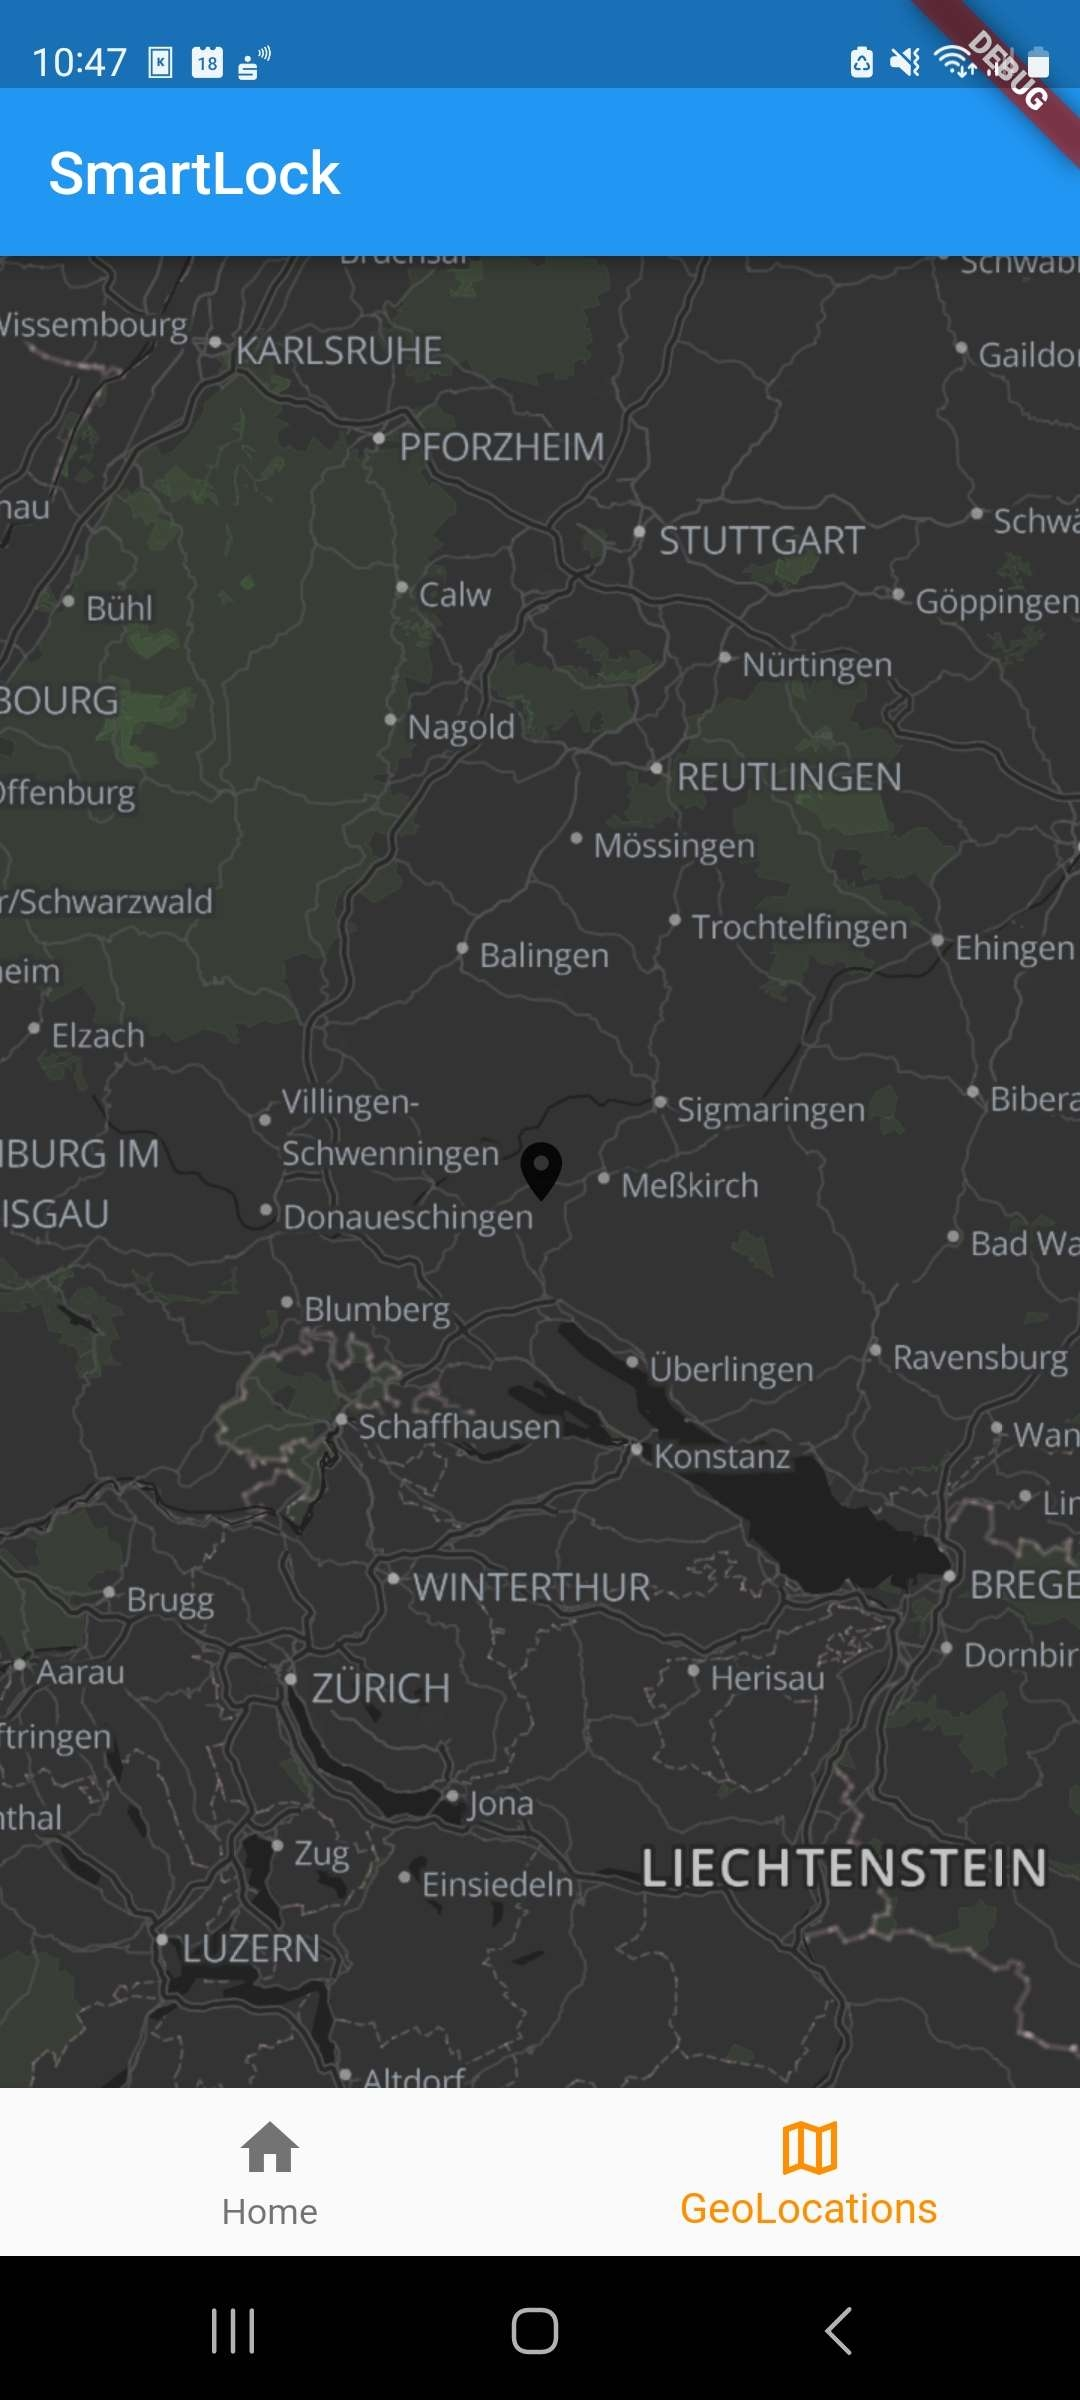
\includegraphics[width=0.3\textwidth]{images/map.jpg}
        \label{fig:map}
    }
    \hfill
    \subfloat[Suche nach Schloss über BLE]{
        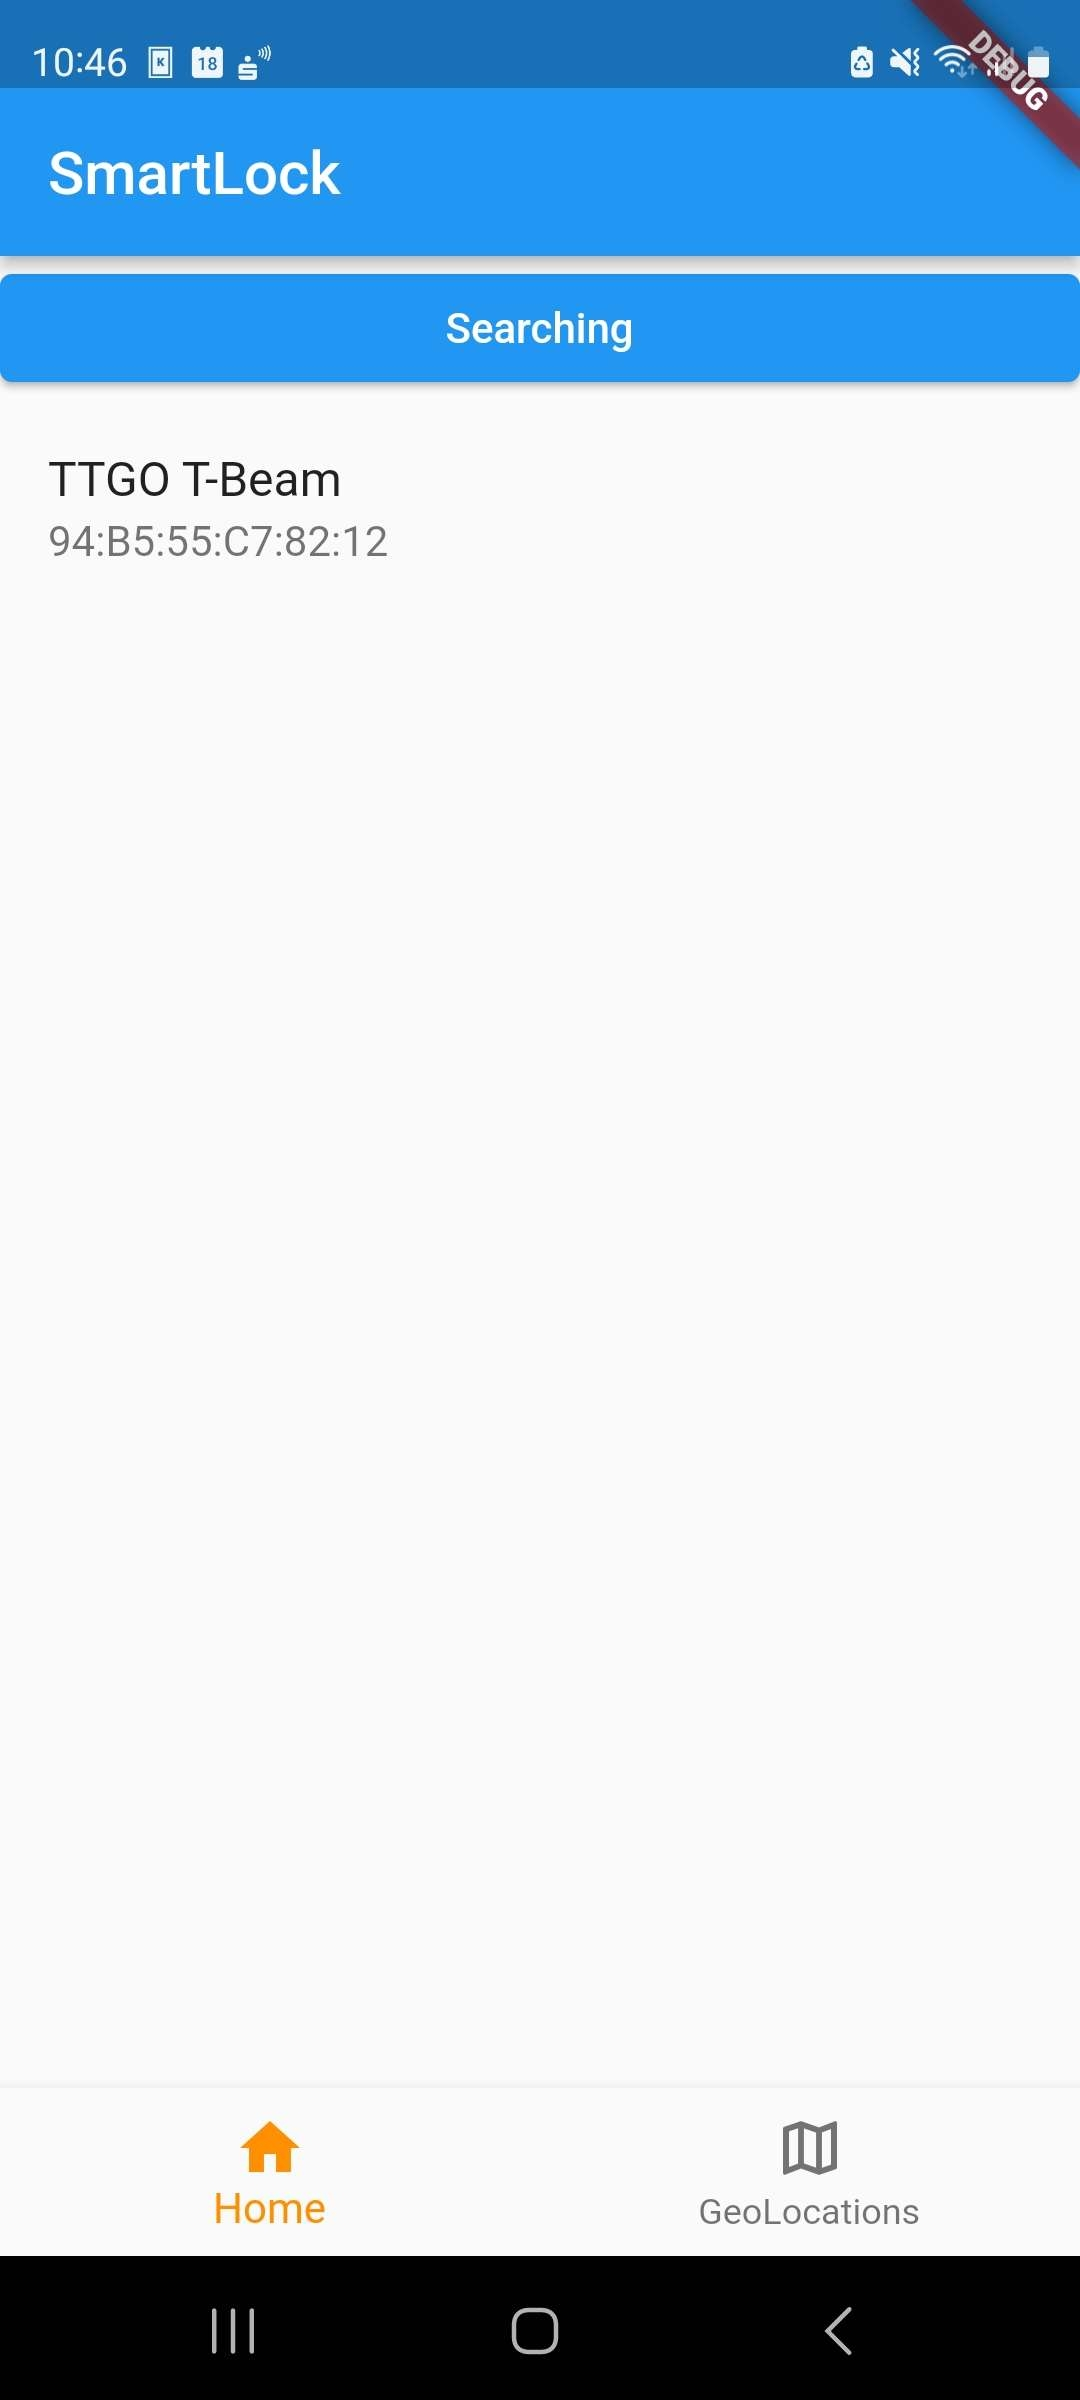
\includegraphics[width=0.3\textwidth]{images/search.jpg}
        \label{fig:search}
        }
    \hfill
    \subfloat[Verbundenes Schloss Öffnen und Schließen]{
        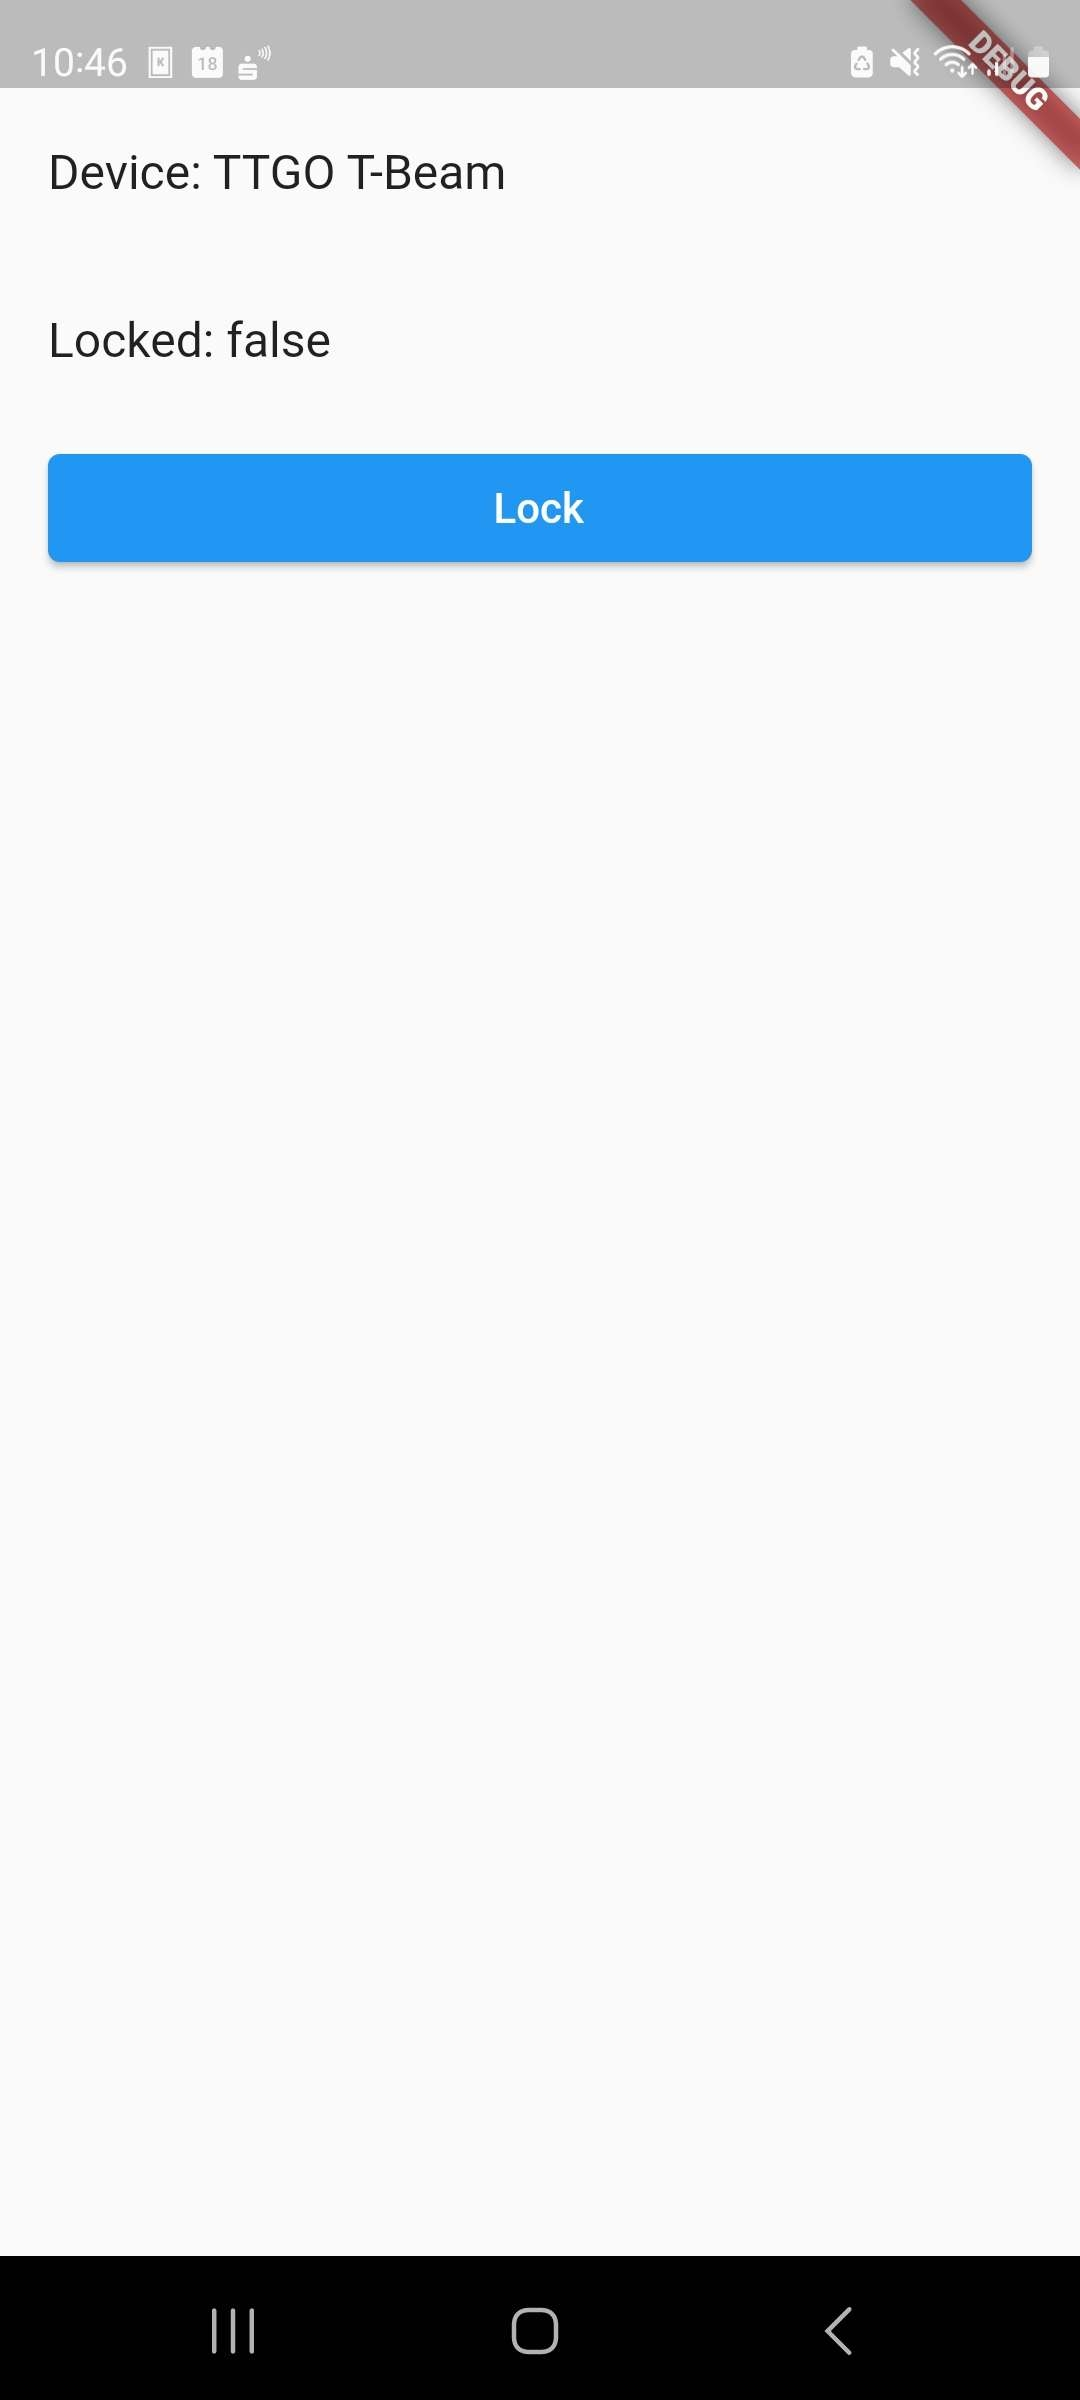
\includegraphics[width=0.3\textwidth]{images/connected.jpg}
        \label{fig:connected}
    }
    \caption{Smart-Lock App: Aufbau}
\end{figure}